\definecolor{ptten}{RGB}{0,0,0}
\definecolor{ptsixgefour}{RGB}{0,114,178}
\definecolor{ptfivegefive}{RGB}{213,94,0}
\definecolor{ptfourgesix}{RGB}{0,158,115}

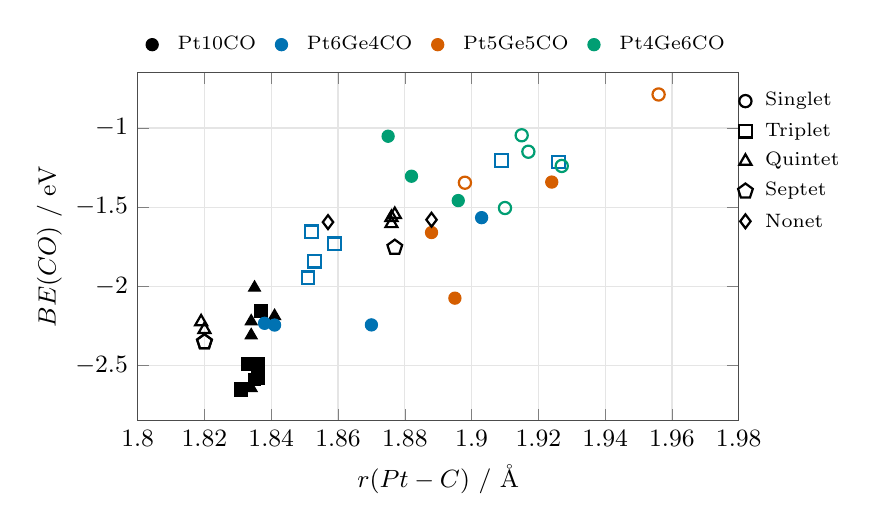
\begin{tikzpicture}
\begin{axis}[
  width=0.76\linewidth,
  height=6.0cm,
  xmin=1.80, xmax=1.98,
  ymin=-2.85, ymax=-0.65,
  xlabel={$r(\ce{Pt-C})$ / \AA},
  ylabel={$BE(\ce{CO})$ / eV},
  ylabel style={yshift=-2pt},
  tick label style={font=\small},
  label style={font=\small},
  grid=major,
  grid style={gray!20},
  axis line style={black!70},
  clip=false,
  legend style={at={(0.5,1.03)},anchor=south,draw=none,inner sep=1pt,
    font=\scriptsize,legend columns=4,column sep=5pt}
]
\addlegendimage{only marks,mark=*,mark size=2.2pt,ptten}
\addlegendentry{\ce{Pt10CO}}
\addlegendimage{only marks,mark=*,mark size=2.2pt,ptsixgefour}
\addlegendentry{\ce{Pt6Ge4CO}}
\addlegendimage{only marks,mark=*,mark size=2.2pt,ptfivegefive}
\addlegendentry{\ce{Pt5Ge5CO}}
\addlegendimage{only marks,mark=*,mark size=2.2pt,ptfourgesix}
\addlegendentry{\ce{Pt4Ge6CO}}
% Filled symbols: crossed-parent models.
\addplot[only marks,mark=square*,mark size=2.3pt,ptten] coordinates {
  (1.831,-2.657) (1.831,-2.650) (1.835,-2.590) (1.836,-2.579)
  (1.833,-2.493) (1.836,-2.493) (1.837,-2.156)};
\addplot[only marks,mark=triangle*,mark size=2.5pt,ptten] coordinates {
  (1.834,-2.645) (1.834,-2.311) (1.834,-2.223) (1.841,-2.189)
  (1.835,-2.010)};
\addplot[only marks,mark=*,mark size=2.2pt,ptsixgefour] coordinates {
  (1.841,-2.246) (1.870,-2.245) (1.838,-2.235) (1.903,-1.567)};
\addplot[only marks,mark=*,mark size=2.2pt,ptfivegefive] coordinates {
  (1.895,-2.076) (1.888,-1.661) (1.924,-1.342)};
\addplot[only marks,mark=*,mark size=2.2pt,ptfourgesix] coordinates {
  (1.896,-1.459) (1.882,-1.305) (1.875,-1.052)};
% Open symbols: models initiated from the global-minimum parent.
\addplot[only marks,mark=triangle,mark size=2.5pt,ptten,
  mark options={fill=white,draw=ptten,line width=0.8pt}] coordinates {
  (1.820,-2.275) (1.819,-2.226) (1.876,-1.605) (1.876,-1.566)
  (1.877,-1.547)};
\addplot[only marks,mark=pentagon,mark size=2.8pt,ptten,
  mark options={fill=white,draw=ptten,line width=0.8pt}] coordinates {
  (1.820,-2.353) (1.820,-2.353) (1.877,-1.755)};
\addplot[only marks,mark=diamond,mark size=2.5pt,ptten,
  mark options={fill=white,draw=ptten,line width=0.8pt}] coordinates {
  (1.857,-1.595) (1.888,-1.580)};
\addplot[only marks,mark=square,mark size=2.3pt,ptsixgefour,
  mark options={fill=white,draw=ptsixgefour,line width=0.8pt}] coordinates {
  (1.851,-1.947) (1.853,-1.842) (1.859,-1.732) (1.852,-1.657)
  (1.926,-1.215) (1.909,-1.207)};
\addplot[only marks,mark=o,mark size=2.2pt,ptfivegefive,
  mark options={fill=white,draw=ptfivegefive,line width=0.8pt}] coordinates {
  (1.898,-1.346) (1.956,-0.788)};
\addplot[only marks,mark=o,mark size=2.2pt,ptfourgesix,
  mark options={fill=white,draw=ptfourgesix,line width=0.8pt}] coordinates {
  (1.910,-1.506) (1.927,-1.240) (1.917,-1.150) (1.915,-1.046)};
% Symbol key: fill is reserved for the structural-parent distinction.
\addplot[only marks,mark=o,mark size=2.2pt,black,
  mark options={fill=white,draw=black,line width=0.8pt}] coordinates {(1.982,-0.83)};
\node[anchor=west,font=\scriptsize] at (axis cs:1.985,-0.83) {Singlet};
\addplot[only marks,mark=square,mark size=2.3pt,black,
  mark options={fill=white,draw=black,line width=0.8pt}] coordinates {(1.982,-1.02)};
\node[anchor=west,font=\scriptsize] at (axis cs:1.985,-1.02) {Triplet};
\addplot[only marks,mark=triangle,mark size=2.5pt,black,
  mark options={fill=white,draw=black,line width=0.8pt}] coordinates {(1.982,-1.21)};
\node[anchor=west,font=\scriptsize] at (axis cs:1.985,-1.21) {Quintet};
\addplot[only marks,mark=pentagon,mark size=2.8pt,black,
  mark options={fill=white,draw=black,line width=0.8pt}] coordinates {(1.982,-1.40)};
\node[anchor=west,font=\scriptsize] at (axis cs:1.985,-1.40) {Septet};
\addplot[only marks,mark=diamond,mark size=2.5pt,black,
  mark options={fill=white,draw=black,line width=0.8pt}] coordinates {(1.982,-1.59)};
\node[anchor=west,font=\scriptsize] at (axis cs:1.985,-1.59) {Nonet};
\end{axis}
\end{tikzpicture}
